\chapter{Uranium Enrichment Regression Results and Discussion}

% https://www.ncbi.nlm.nih.gov/pmc/articles/PMC5554294/

% Although mass spectrometry leads to very accurate analytical results, it has the drawbacks of high costs of the device and its operation involving a long process and destructive sample analysis [1], [2]. https://www.sciencedirect.com/science/article/pii/S1738573317308057#bib1

Verifying the enrichment of HEU through passive nondestructive analysis is important for safeguards applications and homeland security tasks. Nondestructive analysis is preferred to preserve forensics evidence and to allow for remote measurements. 

Measuring the enrichment of uranium is made difficult by the fact that it's characteristic gamma-rays are easily shielded. This task is made more difficult for treaty verification by the restriction placed on inspectors. IAEA inspectors face two major restrictions: a limited amount of time to measure data from declared items and the requirement for an information barrier. This means that direct viewing and analysis of the gamma-ray spectrum - necessary for the enrichment meter method - is impossible. 

The traditional method for using NaI detectors to measure uranium enrichment is the enrichment meter method \cite{Reilly1970}. This method exploits the proportionality between the activity of the 186 keV photon and the enrichment of $^{235}$U. This method requires a 

"Generally, low resolution measurements of 'clean' uranium can be made to 1\% precision over nearly the entire range of uranium enrichment. Measurements in both Europe and the Former Soviet Union have observed bias effects of 5-10\% in low-resolution measurements caused by minor isotopes of uranium. This level of bias has been deemed unacceptable, causing some inspectors to resort to more expensive, time-consuming alternatives like mass spectrometry or liquid-nitrogen-cooler high-resolution detectors. As the international safeguards community attempts to inspect more facilities with less resources, these alternatives become highly undesirable. The minor isotopes come from the use of uranium recycled from reactors being used as feed in the enrichment plants. Daughters of $^{232}$U or $^{236}$U include the thorium decay chain which emits a 238.6-keV gamma ray from $^{212}$Pb. This gamma ray falls in the ROI used to estimate the Compton continuum under the 186-keV gamma ray. In addition, the multitude of high-energy gamma rays from the daughters of $^{232}$U change the shape of the Compton continuum that lies under the desired 186-keV peak. Just to make the entire issue more challenging, the level of this interference varies widely among the samples generally offered to the inspector, causing unpredictable, wide variations in the bias effects" \cite{SPRINKLE1997}

 \cite{VESTERLUND2013}.

Accuracies of +/- 10\% are expected for quick checks of high enriched material while accuracies of +/- 1\% are expected to verify mass spectroscopy measurments \cite{Kull1974}.

% Need to address sample wall effect

NaIGEM code to \cite{MORTREAU2004} 


Changes in background in the facility may affect performance. Studies done measuring uranium enrichment in marine environments have shown that background radiation is important and that existing methods  \cite{Hofstetter2008}.


\begin{equation} \label{eq:uenrichment}
softmax(z_j) = \frac{\exp(z_j)} {\sum_{k=1}^{K} \exp(z_k)}.
\end{equation}

\begin{figure}[H]
	\centering
	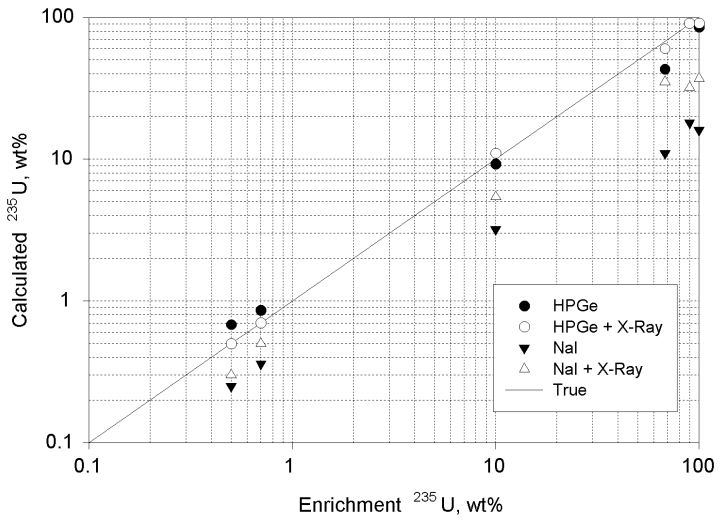
\includegraphics[width=0.99\linewidth]{images/GADRAS_enrichment_hofstetter}
	\caption{Uranium isotopic enrichments calculated from GADRASw analysis of HPGe and NaI spectra with and without additional uranium X-ray component. Reproduced from \cite{Hofstetter2008}}.
	\label{fig:GADRAS_enrichment_hofstetter}
\end{figure}


\section{Problem Description and Training Dataset Overview}

Natural uranium is composed of $^{238}$U, $^{235}$U, and $^{234}$U. 

While $^{238}$U does not have a significant gamma-ray contribution, the $^{234m}$Pa in it's decay chain does. $^{234m}$Pa decay


The software package RadSrc was used to generate the gamma-ray intensities for $^{235}$U and $^{238}$U templates \cite{Hiller2007}. RadSrc, developed at Lawrence Livermore National Laboratory, uses Bateman equations to decay samples. We simulate clean uranium  composed of only $^{235}$U and $^{238}$U. 

We used the F8 tally to calculate the absolute full energy peak efficiency of each energy bin.

Because the uranium x-ray component \cite{Hofstetter2008}.

Additional x-rays may be created from materials around the detector. These are ignored in our analysis.


% FRAM application to U and Pu isotopics https://www.lanl.gov/orgs/n/n1/appnotes/LA-14018-M.pdf

\subsection{Training Datasets}


\begin{table}[H]
\centering
\caption{Range of parameters used for the simple dataset.}
\label{table:hyperparameter_dataset_easy_parameters_enrichment}
\begin{tabular}{ccc}
%\cline{2-3}
 & Hyperparameter Range & Sampling \\ \hline
% \multicolumn{1}{|c|}{Source-Detector Distance {[}cm{]}} & 175.0 & N/A \\ \hline
\multicolumn{1}{c}{Source-Detector Height {[}cm{]}} & 100.0 & N/A\\ % \hline
\multicolumn{1}{c}{FWHM 662 keV {[}s{]}} & 7.5 & N/A \\ % \hline
\multicolumn{1}{c}{\begin{tabular}[c]{@{}c@{}}Shielding \\ (Percent 662 keV Attenuated)\end{tabular}} & 0\%, 20\% & Uniform \\  %\hline
\multicolumn{1}{c}{Integration Time {[}s{]}} & 60 - 3600 & Uniform \\ % \hline
\multicolumn{1}{c}{Linear Calibration Offset} & 0.8 - 1.2 & Uniform \\ % \hline
\multicolumn{1}{c}{Signal to Background Ratio} & 0.5 - 2.0 & Uniform \\ % \hline
\end{tabular}
\end{table}


\begin{table}[H]
\centering
\caption{Range of parameters used for the full dataset.}
\label{table:hyperparameter_dataset_full_parameters_enrichment}
\begin{tabular}{ccc}
% \cline{2-3}
 & Hyperparameter Range & Sampling \\ \hline
\multicolumn{1}{c}{Source-Detector Distance {[}cm{]}} & 50.5, 175.0, 300 & Uniform \\ % \hline
\multicolumn{1}{c}{Source-Detector Height {[}cm{]}} & 50, 100.0, 150 & Uniform \\ % \hline
\multicolumn{1}{c}{FWHM 662 keV {[}s{]}} & 7.0, 7.5, 8.0 & Uniform \\ % \hline
\multicolumn{1}{c}{\begin{tabular}[c]{@{}c@{}}Shielding\\ (Percent 662 keV Attenuated)\end{tabular}} & 0\%, 20\%, 40\%, 60\% & Uniform \\ % \hline
\multicolumn{1}{c}{Reprocessing isotopes} & $^{232}$U, $^{236}$U & Uniform \\ % \hline
\multicolumn{1}{c}{Integration Time {[}s{]}} & 60 - 3600 & Uniform \\ % \hline
\multicolumn{1}{c}{Linear Calibration Offset} & 0.8 - 1.2 & Uniform \\ % \hline
\multicolumn{1}{c}{Signal to Background Ratio} & 0.5 - 2.0 & Uniform \\ % \hline
\end{tabular}
\end{table}


\subsection{Autoencoder Performance - Fine Tuning networks on Urban Source Search Versus Uranium Enrichment Datasets}

This section will compare performance differences when fine tuning an autoencoder using features found from the urban source search and the uranium enrichment datasets. The task of isotope identification in the urban source search dataset is different from the task of quantifying uranium enrichment in the uranium enrichment dataset. If the features found from the urban source search are useful as pretraining for uranium enrichment, pretrained networks may be distributed to the community.


networks and as feature extractors for a DNN. To do this, a trained CAE and DAE will be connected to a dense network. These will be trained to either fixing the autoencoder's weights or by fine-tuning them while the network learns.


\section{Generalization Results - Simulated Data}

These sections describe how each model performed on simulated enriched uranium.


\begin{table}[H]
\centering
\label{table:generalization_enrichment_values}
\caption{$^{235}$U enrichment values.}
\begin{tabular}{c}
\hline
0.10 \\ \hline
0.25 \\ \hline
0.50 \\ \hline
0.75 \\ \hline
0.85 \\ \hline
0.90 \\ \hline
0.95 \\ \hline
\end{tabular}
\end{table}


\subsection{Generalization Results on Shielding}

Enriched uranium spectra were simulated with various amounts of shielding.



\begin{figure}[H]
     \centering
     \begin{subfigure}[b]{0.9\textwidth}
         \centering
         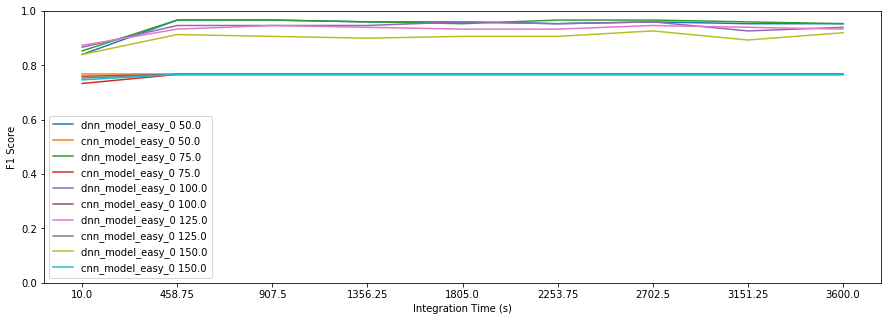
\includegraphics[width=\textwidth]{images/results_easy_distance_comparison}
         \caption{Simple Dataset.}
         \label{fig:results_full_background_inject_simple}
     \end{subfigure}

     \begin{subfigure}[b]{0.9\textwidth}
         \centering
         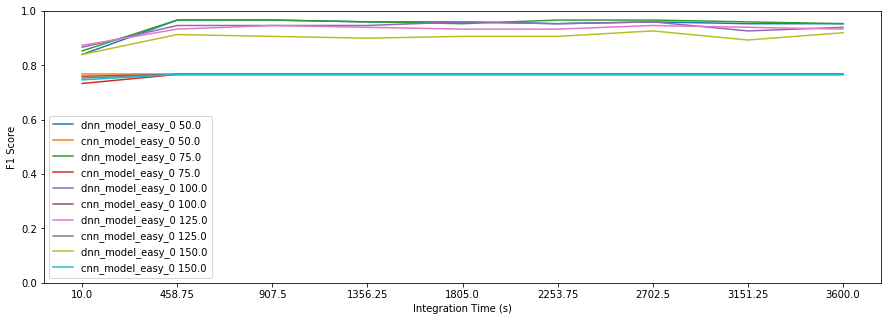
\includegraphics[width=\textwidth]{images/results_easy_distance_comparison}
         \caption{Full Dataset.}
         \label{fig:results_full_background_inject_full}
     \end{subfigure}
        \caption{Absolute error for all models trained on the full dataset. Datasets included here used various amounts of shielding.}
        \label{fig:results_full_background_inject}
\end{figure}



\subsection{Generalization Results on Changing Calibration}

Unshielded enriched uranium spectra were simulated with various changes in their gain.  


\begin{figure}[H]
     \centering
     \begin{subfigure}[b]{0.9\textwidth}
         \centering
         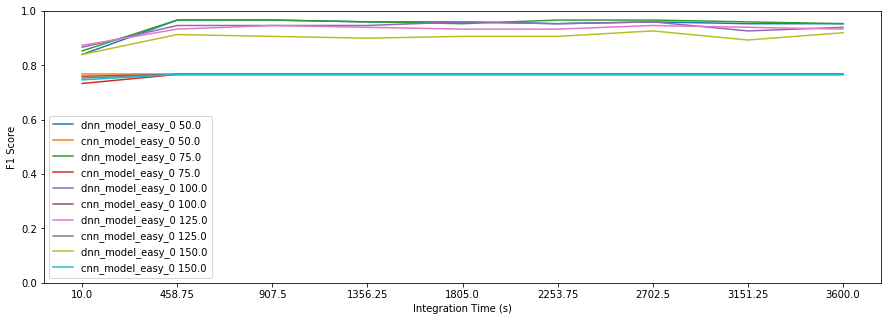
\includegraphics[width=\textwidth]{images/results_easy_distance_comparison}
         \caption{Simple Dataset.}
         \label{fig:results_full_background_inject_simple}
     \end{subfigure}

     \begin{subfigure}[b]{0.9\textwidth}
         \centering
         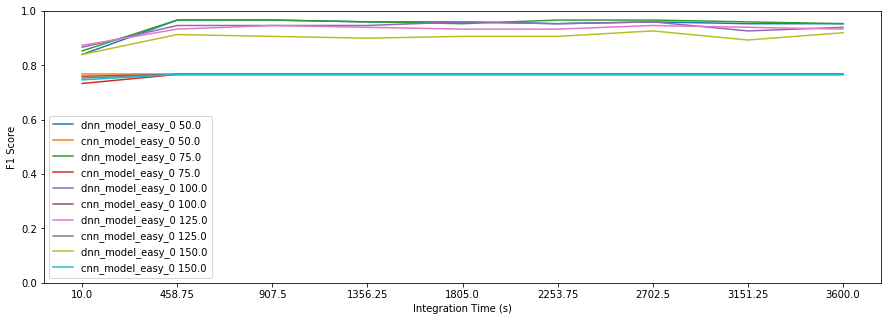
\includegraphics[width=\textwidth]{images/results_easy_distance_comparison}
         \caption{Full Dataset.}
         \label{fig:results_full_background_inject_full}
     \end{subfigure}
        \caption{Absolute error for all models trained on the full dataset. Datasets included here used various amounts of shielding.}
        \label{fig:results_full_background_inject}
\end{figure}


\subsection{Generalization Results on Changing Background}

Unshielded enriched uranium spectra were simulated with various background templates.  


\begin{figure}[H]
     \centering
     \begin{subfigure}[b]{0.9\textwidth}
         \centering
         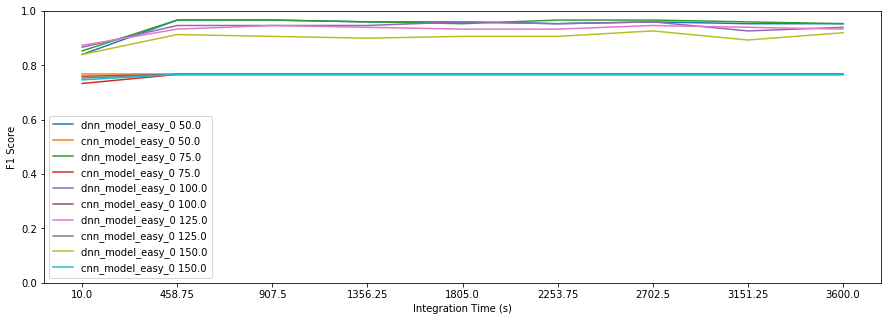
\includegraphics[width=\textwidth]{images/results_easy_distance_comparison}
         \caption{Simple Dataset.}
         \label{fig:results_full_background_inject_simple}
     \end{subfigure}

     \begin{subfigure}[b]{0.9\textwidth}
         \centering
         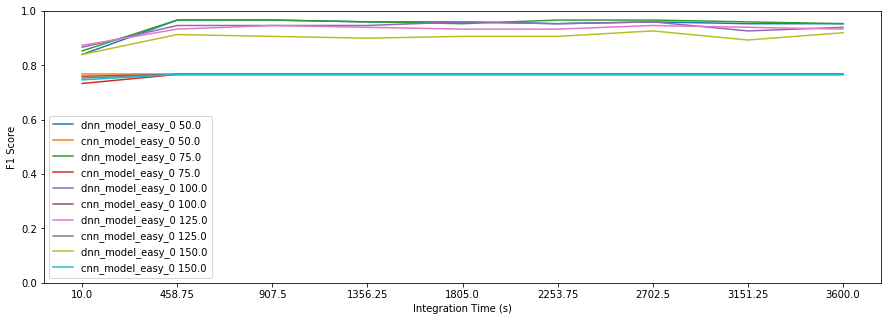
\includegraphics[width=\textwidth]{images/results_easy_distance_comparison}
         \caption{Full Dataset.}
         \label{fig:results_full_background_inject_full}
     \end{subfigure}
        \caption{Absolute error for all models trained on the full dataset. Datasets included here used various background templates.}
        \label{fig:results_full_background_inject}
\end{figure}


\subsection{Generalization Results on Reprocessed Uranium}

Reprocessed uranium contains trace parasitic impurities ($^{233}$U, $^{236}$U, $^{237}$Np, $^{239}$Pu) that can change the gamma-ray spectrum and interfere with the 186 keV gamma-ray from $^{235}$U. To test the effect of these on 


\begin{figure}[H]
     \centering
     \begin{subfigure}[b]{0.9\textwidth}
         \centering
         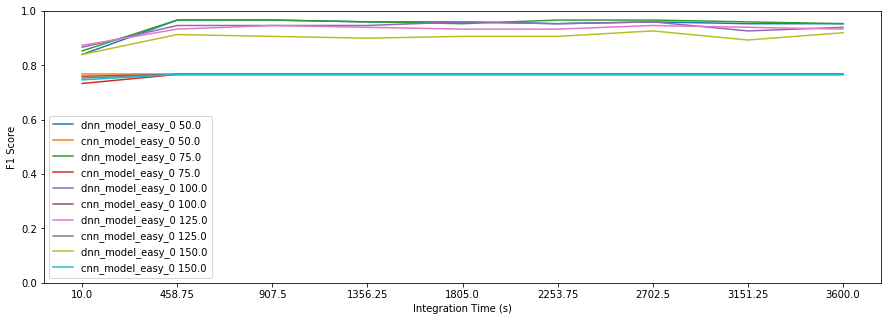
\includegraphics[width=\textwidth]{images/results_easy_distance_comparison}
         \caption{Simple Dataset.}
         \label{fig:results_full_background_inject_simple}
     \end{subfigure}

     \begin{subfigure}[b]{0.9\textwidth}
         \centering
         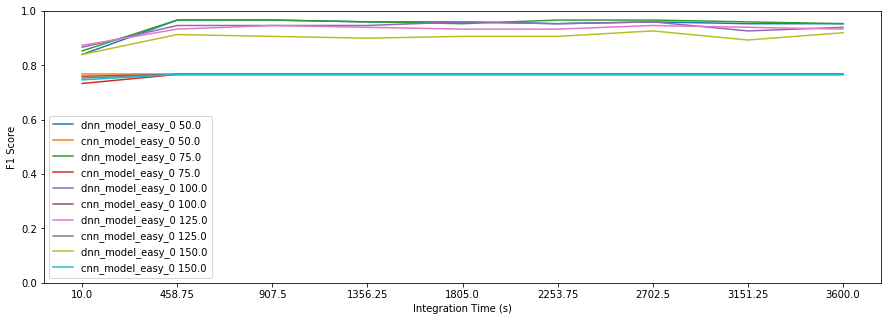
\includegraphics[width=\textwidth]{images/results_easy_distance_comparison}
         \caption{Full Dataset.}
         \label{fig:results_full_background_inject_full}
     \end{subfigure}
        \caption{Absolute error for all models trained on the full dataset. Datasets included here used various background templates.}
        \label{fig:results_full_background_inject}
\end{figure}


\section{Results - Rocky Flats Shells}


% Is it necessary to re-run the hyperparameter search, or are the 'simple' models good enough?

The reported Rocky Flats shells isotopics are shown in Table \ref{table:rockyflats_isotopics}. Recent work has found estimated that impurities of $^{232}$U, mass fraction 6.0E-9\%, and $^{237}$Np, mass fraction 1.8E-4\%, \cite{RawoolSullivan2012} existed in the shells in 1971 (the year the shells were fabricated).

\begin{table}[H]
\centering
\caption{Rocky Flats Isotopics \cite{Rothe1997}.}
\label{table:rockyflats_isotopics}
\begin{tabular}{|c|c|}
\hline
Uranium Isotope & \begin{tabular}[c]{@{}c@{}}Weight Percentage\\ (1965)\end{tabular} \\ \hline
$^{233}$U & - \\ \hline
$^{234}$U & 1.00 \\ \hline
$^{235}$U & 93.19 \\ \hline
$^{236}$U & 0.4 \\ \hline
$^{238}$U & 5.41 \\ \hline
\end{tabular}
\end{table}

Asymptotic models are 


Again, measure asymptotic MSE convergence.



\section{Results from Adding Physics}

Show how accuracy changes when using
\begin{itemize}
    \item Multiple detector-source distance
    \subitem CNN, DNN, BS-DAE, BS-CAE, V-DAE, BS-CAE
    \item Cement floor
    \subitem CNN, DNN, BS-DAE, BS-CAE, V-DAE, BS-CAE
    \item Solid vs shell vs solid and shell uranium
    \subitem CNN, DNN, BS-DAE, BS-CAE, V-DAE, BS-CAE
    \item 
\end{itemize}







